\documentclass{article}
\usepackage[margin=1in]{geometry}
\usepackage{problemset}
\showsolntrue

% Custom commands
\newcommand{\R}{\mathbb{R}}
\newcommand{\X}{\mathcal{X}}
\newcommand{\Y}{\mathcal{Y}}
\newcommand{\E}{\mathbb{E}}
\newcommand{\V}{\text{Var}}
\renewcommand{\P}{\mathbb{P}}

\begin{document}

\pstitle{%
    MATH 189%
}{
    Homework 3%
}[due Wednesday, February 4 at 8:00AM]

\textbf{Resources:} These problems appear in Chs. 4-5 of the textbook pgs. 193-199 and 224-228.

\textbf{Format requirements:} Type your homeworks using \LaTeX with embedded plots for the applied exercises.

\textbf{Grading:} The grading is based 50\% on correctness and 50\% on correctness.

\vspace{1em}

\begin{probset}

% --- Problem 1 ---
\begin{prob}[\textbf{Ch. 4 conceptual exercise 7}]
    Suppose that we wish to predict whether a given stock will issue a dividend this year (“Yes” or “No”) based on $X$, last year's percent profit. We examine a large number of companies and discover that the mean value of $X$ for companies that issued a dividend was $\bar{X} = 10$, while the mean for those that didn't was $\bar{X} = 0$. In addition, the variance of $X$ for these two sets of companies was $\hat{\sigma}^2 = 36$. Finally, 80\% of companies issued dividends. Assuming that $X$ follows a normal distribution, predict the probability that a company will issue a dividend this year given that its percentage profit was $X = 4$ last year.

    \begin{soln}
        Using Bayes' theorem, we can find the probability that a company will issue a dividend this year given that its percentage profit was $X = 4$ last year. We know that $P(Y = \text{Yes}) = 0.8$ and $P(Y = \text{No}) = 0.2$. We also know that $P(X = 4 | Y = \text{Yes}) = \frac{1}{72\pi} e^{-\frac{(4 - 10)^2}{72}} \approx 0.00268$ and $P(X = 4 | Y = \text{No}) = \frac{1}{72\pi} e^{-\frac{(4 - 0)^2}{72}} \approx 0.00354$. Thus,

        \[
            P(Y = \text{Yes} | X = 4) = \frac{P(X = 4 | Y = \text{Yes}) P(Y = \text{Yes})}{P(X = 4)} = \frac{0.00268 \cdot 0.8}{0.00268 \cdot 0.8 + 0.00354 \cdot 0.2} \approx 0.752
        \]

        So the probability that a company will issue a dividend this year given that its percentage profit was $X = 4$ last year is approximately 0.752.
    \end{soln}
\end{prob}

% --- Problem 2 ---
\begin{prob}[\textbf{Ch. 4 conceptual exercise 8}]
    Suppose that we take a data set, divide it into equally-sized training and test sets, and then try out two different classification procedures. First we use logistic regression and get an error rate of 20\% on the training data and 30\% on the test data. Next we use 1-nearest neighbors (i.e. $K = 1$) and get an average error rate (averaged over both test and training data sets) of 18\%. Based on these results, which method should we prefer to use for classification of new observations? Why?

    \begin{soln}
        We should prefer logistic regression for classification of new observations. The test error rate of 30\% is more promising than the average error rate of 18\% for 1-nearest neighbors ($K = 1$) because 1-NNs will generally overfit since they only care about one neighbor, usually achieving close to 0\% training error. This indicates that the test error rate is closer to 36\% which is worse than the 30\% for logistic regression.
    \end{soln}
\end{prob}

\newpage

% --- Problem 3 ---
\begin{prob}[\textbf{Ch. 5 conceptual exercise 3}]
    We now review $k$-fold cross-validation.

    \begin{subprobset}
    \begin{subprob}
        Explain how $k$-fold cross-validation is implemented.

        \begin{soln}
            $k$-fold cross-validation is implemented by dividing the data into $k$ equally sized folds. Then, for each fold, we train the model on the remaining $k-1$ folds and test on the fold. We then average the error rates over all $k$ folds.
        \end{soln}
    \end{subprob}
    
    \begin{subprob}
        What are the advantages and disadvantages of $k$-fold cross-validation relative to:

        \begin{enumerate}[label=\roman*.]
            \item The validation set approach?
            \item Leave-one-out cross-validation?
        \end{enumerate}

        \begin{soln}
            $k$-fold cross-validation is more efficient than leave-one-out cross-validation because you're not training on each data point $n-1$ times for $n$ data points. A disadvantage is that it may not be as accurate as leave-one-out cross-validation because certain folds may be more representative of the data than others and will hence bias the results.
            
            $k$-fold cross-validation is also more accurate than the validation set approach because it ultimately tests on all of the data points, not just a subset. A disadvantage is that it is more computationally expensive than the validation set approach because you're training on $k-1$ times per data point for $k$ folds.
        \end{soln}
    \end{subprob}
    \end{subprobset}
\end{prob}

\newpage

% --- Problem 4 ---
\begin{prob}[\textbf{Ch. 4 applied exercise 16}]
    Using the \texttt{Boston} data set, fit classification models in order to predict whether a given suburb has a crime rate above or below the median. Explore logistic regression, LDA, naive Bayes, and KNN models using various subsets of the predictors. Describe your findings. Hint: You will have to create the response variable yourself, using the variables that are contained in the \texttt{Boston} data set.

    \begin{soln}
        \begin{center}
            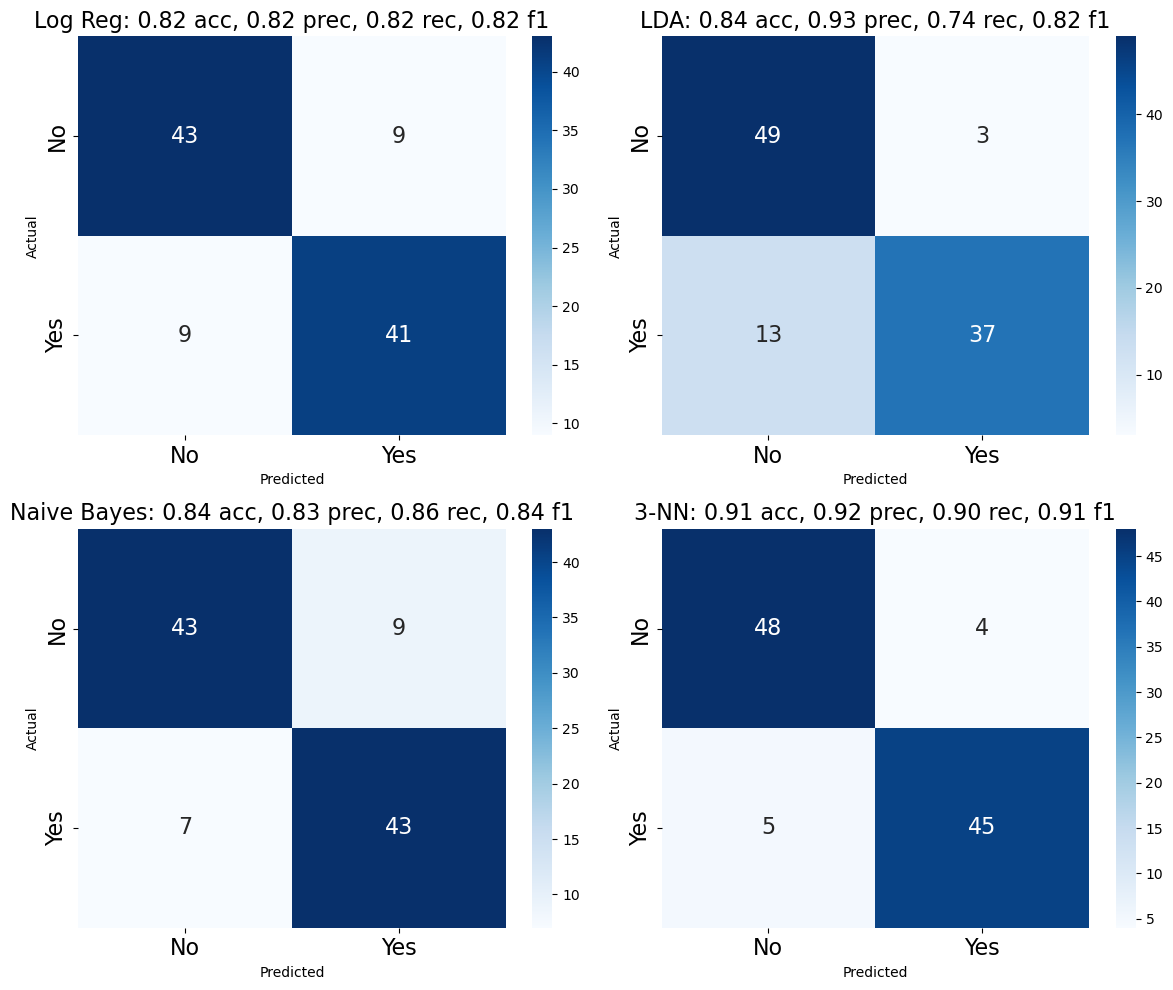
\includegraphics[width=0.65\textwidth]{Images/4.1.png}
        \end{center}
        This confusion matrix is from all the predictors. As you can see from the confusion matrices and the metrics, Log Reg and Naive Bayes perform about equally well with all metrics being around 0.82-0.84 with NB being slightly better.

        LDA performs better in terms of precision (0.93) but worse in recall (0.74). The F1 score is about the same being 0.82 so LDA is the choice if you need low false positives. The 3-NN performs the best overall with all metrics being 0.90 or higher.

        \begin{center}
            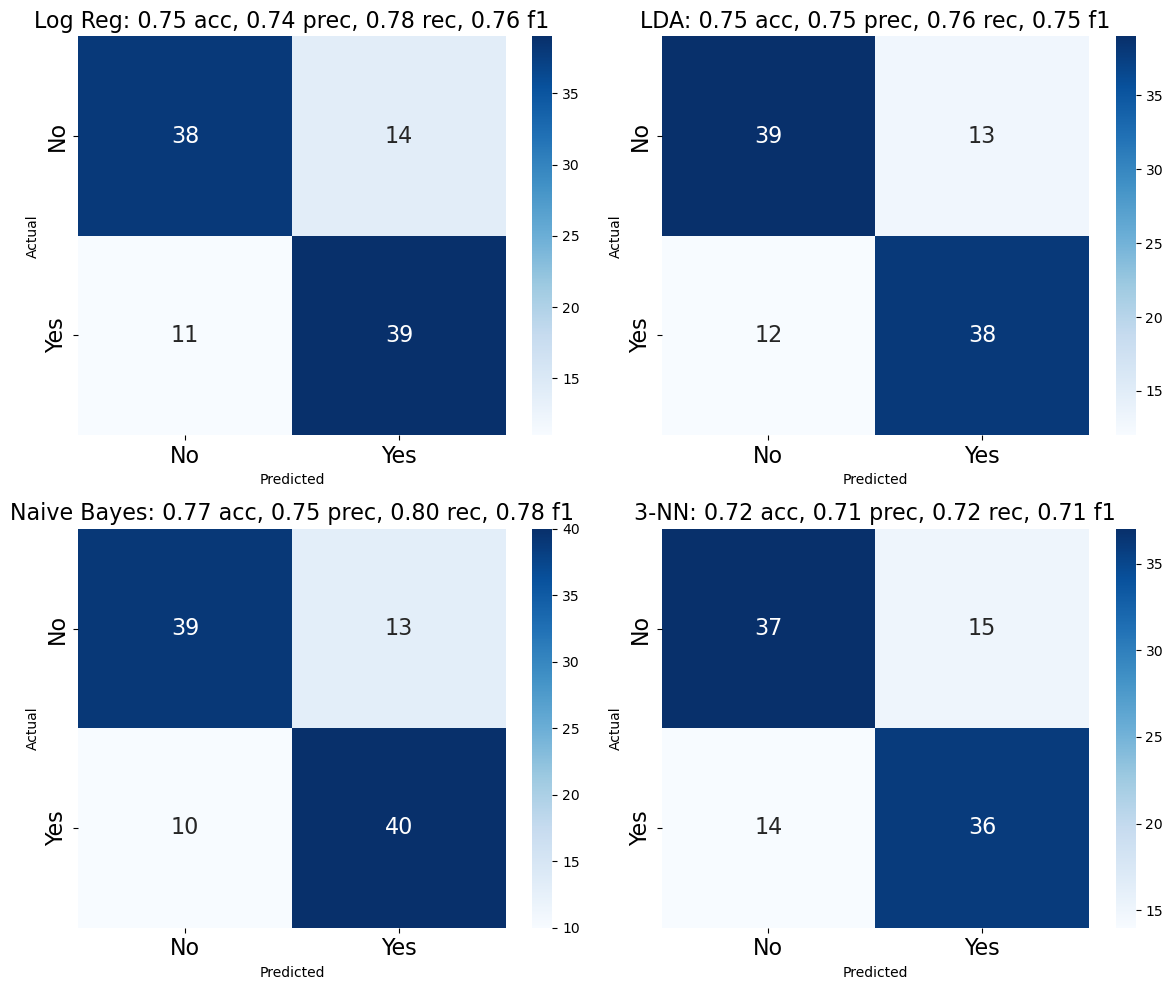
\includegraphics[width=0.65\textwidth]{Images/4.2.png}
        \end{center}
        This confusion matrix is from the socioeconomic predictors, i.e. \texttt{lstat}, \texttt{medv}, and \texttt{ptratio}. In this case, the 3-NN performs the worst overall indicating that whatever gave it the edge before wasn't a socioeconomic predictor.

        LDA and Log Reg perform about equally well with all metrics being around 0.74-0.78 with Log Reg having an edge with recall being 0.78. Overall, Naive Bayes performs the best overall with metrics running from 0.75-0.80 with particular emphasis on recall being 0.80.

        \begin{center}
            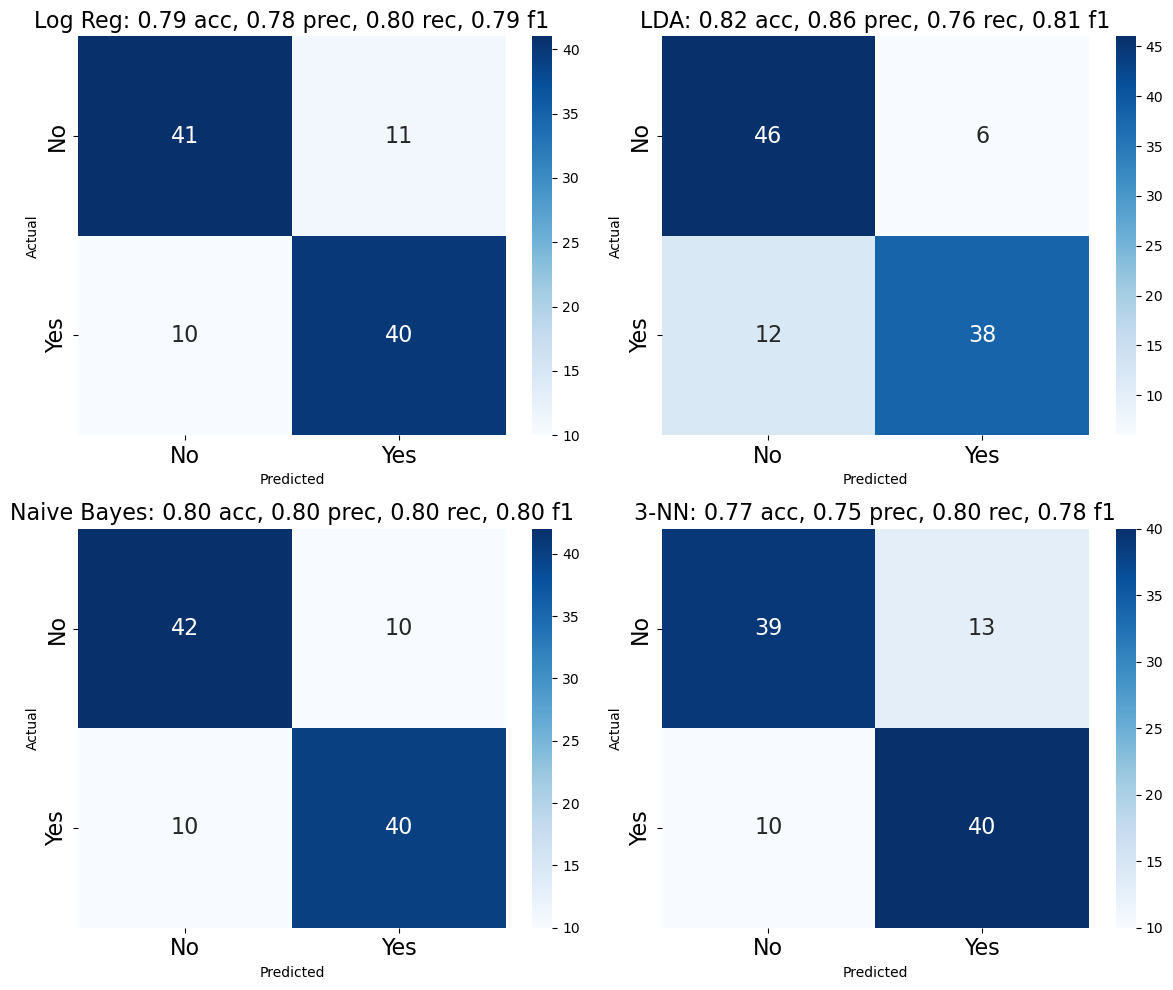
\includegraphics[width=0.65\textwidth]{Images/4.3.png}
        \end{center}
        This confusion matrix is from the location predictors, i.e. \texttt{dis}, \texttt{nox}, and \texttt{chas}. In this case, Naive Bayes and Log Reg perform about equally. LDA is back to having high precision (0.86) but low recall (0.76). The 3-NN also performed relatively poorly. Overall, these predictors surprisingly performed a bit better than the socioeconomic predictors indicating that location is more important in predicting crime rate.
    \end{soln}
\end{prob}

\newpage

% --- Problem 5 ---
\begin{prob}[\textbf{Ch. 5 applied exercise 9}]
    We will again consider the \texttt{Boston} housing data set, from the ISLP library.

    \begin{subprobset}
    \begin{subprob}
        Based on this data set, provide an estimate for the population mean of \texttt{medv}. Call this estimate $\hat{\mu}$.

        \begin{soln}
            We predict $\hat{\mu} = 22.5328$ for the population mean of \texttt{medv}.
        \end{soln}
    \end{subprob}

    \begin{subprob}
        Provide an estimate of the standard error of $\hat{\mu}$. Interpret this result. Hint: We can compute the standard error of the sample mean by dividing the sample standard deviation by the square root of the number of observations.

        \begin{soln}
            We estimate the standard error of $\hat{\mu}$ to be 0.4089. This means that the sample mean is likely to be within 0.4089 of the true population mean.
        \end{soln}
    \end{subprob}

    \begin{subprob}
        Now estimate the standard error of $\hat{\mu}$ using the bootstrap. How does this compare to your answer from (b)?

        \begin{soln}
            \begin{center}
                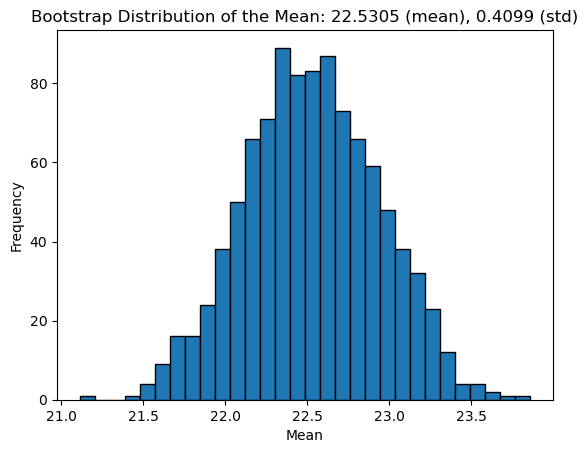
\includegraphics[width=0.65\textwidth]{Images/5c.png}
            \end{center}
            The bootstrap estimate of the standard error of $\hat{\mu}$ is 0.4099 which is very close to the answer from (b) since it's only off by 0.001.
        \end{soln}
    \end{subprob}

    \begin{subprob}
        Based on your bootstrap estimate from (c), provide a 95\% confidence interval for the mean of \texttt{medv}. Compare it to the results obtained by using \texttt{Boston['medv'].std()} and the two standard error rule. Hint: You can approximate a 95\% confidence interval using the formula $[\hat{\mu} - 2 SE(\hat{\mu}), \hat{\mu} + 2 SE(\hat{\mu})]$.

        \begin{soln}
            Using the bootstrap estimate, the 95\% confidence interval is $22.5305 \pm 2(0.4099) = [21.7107, 23.3503]$. Using our results from (b), the 95\% confidence interval is $22.5328 \pm 2(0.4089) = [21.7150, 23.3506]$. These intervals are extremely similar and only differ by less than 0.01.
        \end{soln}
    \end{subprob}

    \newpage

    \begin{subprob}
        Based on this data set, provide an estimate, $\hat{\mu}_{med}$, for the median value of \texttt{medv} in the population.

        \begin{soln}
            We predict $\hat{\mu}_{med} = 21.2$ for the median value of \texttt{medv} in the population.
        \end{soln}
    \end{subprob}

    \begin{subprob}
        We now would like to estimate the standard error of $\hat{\mu}_{med}$. Unfortunately, there is no simple formula for computing the standard error of the median. Instead, estimate the standard error of the median using the bootstrap. Comment on your findings.

        \begin{soln}
            \begin{center}
                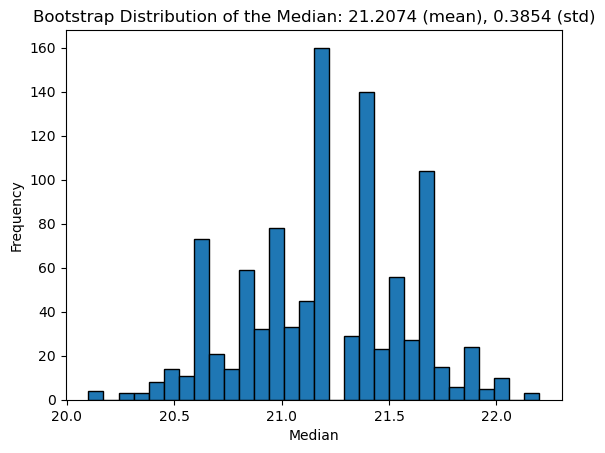
\includegraphics[width=0.65\textwidth]{Images/5f.png}
            \end{center}
            The bootstrap estimate of the standard error of $\hat{\mu}_{med}$ is 0.3854. This is smaller than the standard error of $\hat{\mu}$ indicating that the median is more stable than the mean. This makes sense since the median is not as affected by outliers as the mean.
        \end{soln}
    \end{subprob}
    
    \newpage

    \begin{subprob}
        Based on this data set, provide an estimate for the tenth percentile of \texttt{medv} in Boston census tracts. Call this quantity $\hat{\mu}_{0.1}$. (You can use the \texttt{np.percentile()} function.)

        \begin{soln}
            We predict $\hat{\mu}_{0.1} = 12.75$ for the tenth percentile of \texttt{medv} in the population.
        \end{soln}
    \end{subprob}

    \begin{subprob}
        Use the bootstrap to estimate the standard error of $\hat{\mu}_{0.1}$. Comment on your findings

        \begin{soln}
            \begin{center}
                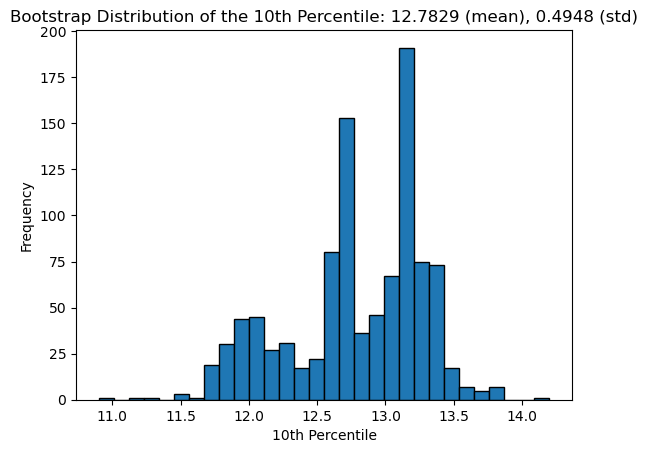
\includegraphics[width=0.65\textwidth]{Images/5h.png}
            \end{center}
            Interestingly, the bootstrap estimate of the standard error of $\hat{\mu}_{0.1}$ is 0.4948 which is even larger than the standard error of the mean. This does make somewhat sense though since there will be more variablility in the tails of the distribution than the center.
        \end{soln}
    \end{subprob}
    \end{subprobset}
\end{prob}
\end{probset}
\end{document}